\documentclass[oneside, 10pt]{article}
\usepackage[margin=1.2in]{geometry}
\usepackage[english]{babel}
\usepackage{amsfonts}
\usepackage{amsmath}
\usepackage{amssymb}
\usepackage{minted}
\usepackage[utf8]{inputenc}
\usepackage[T1]{fontenc}
\usepackage{listings}
\usepackage{subfig}
\usepackage[pdfencoding=auto, psdextra]{hyperref}
\usepackage[
    type={CC},
    modifier={by-nc-sa},
    version={4.0},
]{doclicense}

\title{\LARGE CSC258 PRELAB \#4}
\author{\href{https://tingfengx.github.io}{Tingfeng Xia}}
\date{\today}
\begin{document}
\maketitle
\section*{PART I}
\paragraph{1.} Here is my logic gate level schematic
\begin{center}
    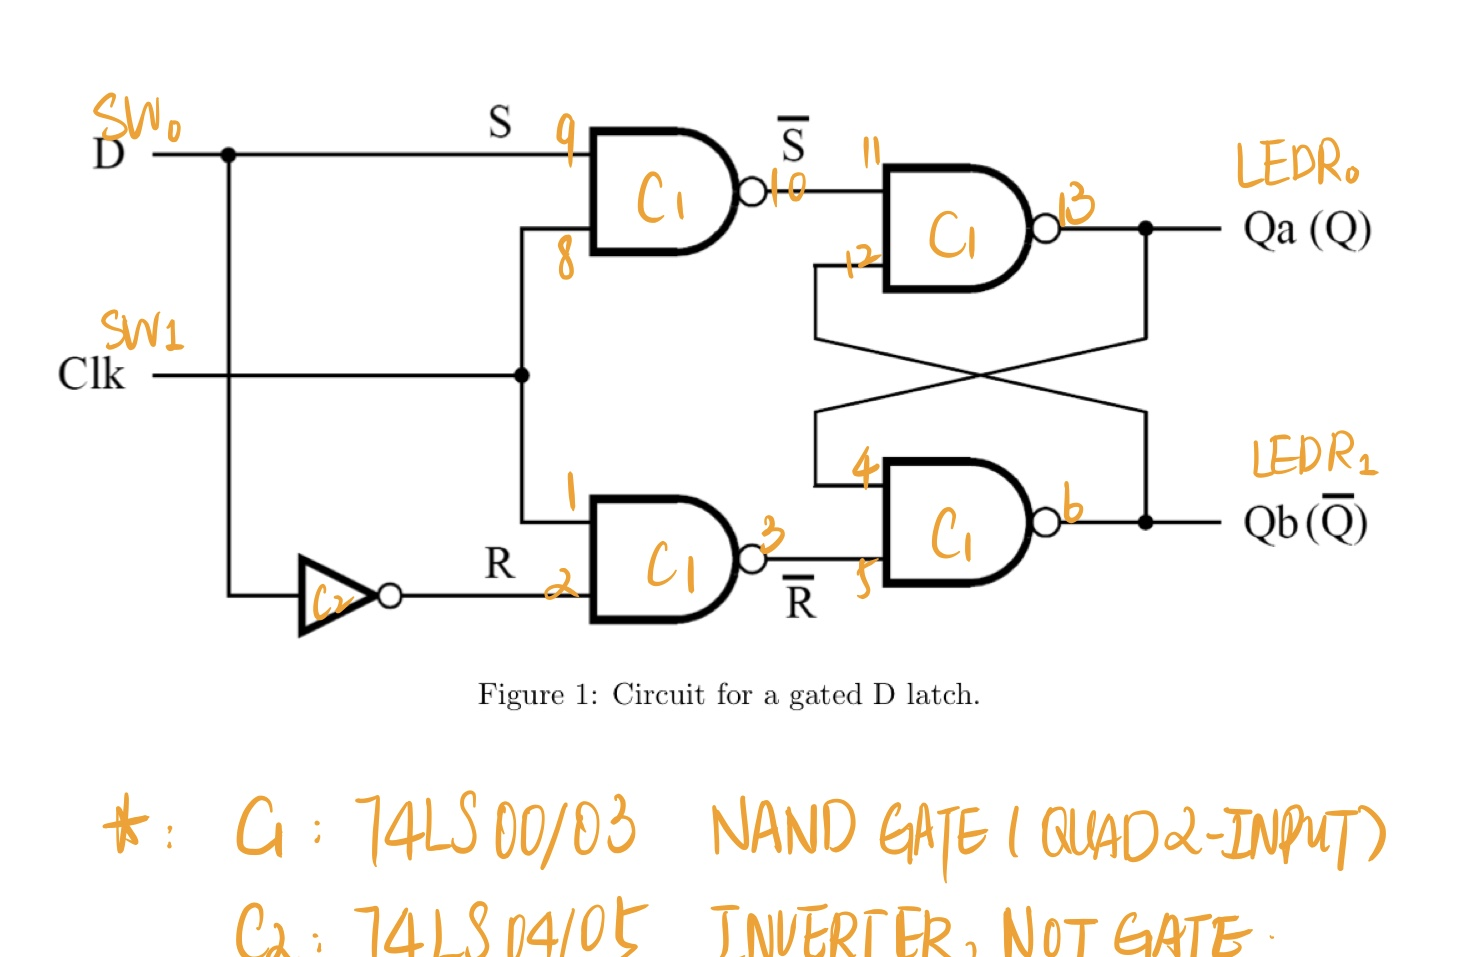
\includegraphics[scale=0.21]{q1_scheme.jpg}
\end{center}
\paragraph{4.} To avoid uncertainty, we shall avoid any case where $Clk\gets 0$ 
at initial state. Since $D$ is unspecified, the behavior of the circuit can be 
unpredictable. 

\section*{PART II}
\paragraph{1.} Here is my code for RegisterALU:
\begin{minted}{verilog}
    module RegisterALU(SW, KEY, LEDR, HEX0, HEX1, HEX2, HEX3, HEX4, HEX5);
        input [9:0] SW;
        input [0:0] KEY;
        output [6:0] HEX0;
        output [6:0] HEX1;
        output [6:0] HEX2;
        output [6:0] HEX3;
        output [6:0] HEX4;
        output [6:0] HEX5;
        output [7:0] LEDR;
            
        reg [7:0] ALUout;
        reg [7:0] Register;
        
        wire [3:0] A;
        wire [3:0] B;
        assign A[3:0] = SW[3:0];
        assign B[3:0] = Register[3:0];
        
        // two wires for arithmetic operations
        wire [4:0] addOneToA;
        wire [4:0] addAToB;
        
        // two 4 bit ripple adders 
        rippleadder4 ra1(
            .SW({1'b0, A[3:0], 4'b0001}), 
            .LEDR(addOneToA[4:0])  // output five bit wire
        );
        rippleadder4 ra2(
            .SW({1'b0, A[3:0], B[3:0]}), 
            .LEDR(addAToB[4:0]) // the output five bit wire
        );
        
        always @(*)
        begin
            case (SW[7:5])
                3'b000: ALUout[7:0] = {3'b000, addOneToA[4:0]};
                3'b001: ALUout[7:0] = {3'b000, addAToB[4:0]};
                3'b010: ALUout[7:0] = {3'b000, A[3:0] + B[3:0]};
                3'b011: ALUout[7:0] = {A[3:0] | B[3:0], A[3:0] ^ B[3:0]};
                3'b100: ALUout[7:0] = (| {A[3:0], B[3:0]}) ? 8'b00000001 : 8'b00000000;
                3'b101: ALUout[7:0] = B[3:0] << A[3:0];
                3'b110: ALUout[7:0] = B[3:0] >> A[3:0];
                3'b111: ALUout[7:0] = A[3:0] * B[3:0];
                default: ALUout[7:0] = 8'b11111111; //meaningless number, indicate fall back.
            endcase
        end
        
        always @(posedge KEY[0])
        begin
            if (SW[9] == 1'b0) // SW[9 for reset_n]
                Register[7:0] <= 8'b00000000;
            else
                Register[7:0] <= ALUout[7:0];
        end
        
        assign LEDR[7:0] = ALUout[7:0];
        
        // display nothing
        assign HEX1[6:0] = 7'b1111111;
        assign HEX2[6:0] = 7'b1111111;
        assign HEX3[6:0] = 7'b1111111;
        // HEX0 display the input A
        hexdecoder hex0(
            .SW(A[3:0]),
            .HEX(HEX0[6:0])
        );
        // HEX4 display lower four bits of register
        hexdecoder hex4(
            .SW(Register[3:0]),
            .HEX(HEX4[6:0])
        );
        // HEX5 display higher four bits of register
        hexdecoder hex5(
            .SW(Register[7:4]),
            .HEX(HEX5[6:0])
        );
    endmodule

    module hexdecoder(HEX, SW);
        input [3:0] SW;
        output [6:0] HEX;

        hex0 u0(
            .x(SW[3]),
            .y(SW[2]),
            .z(SW[1]),
            .w(SW[0]),
            .m(HEX[0])
        );
        
        hex1 u1(
            .x(SW[3]),
            .y(SW[2]),
            .z(SW[1]),
            .w(SW[0]),
            .m(HEX[1])
        );
        
        hex2 u2(
            .x(SW[3]),
            .y(SW[2]),
            .z(SW[1]),
            .w(SW[0]),
            .m(HEX[2])
        );

        hex3 u3(
            .x(SW[3]),
            .y(SW[2]),
            .z(SW[1]),
            .w(SW[0]),
            .m(HEX[3])
        );

        hex4 u4(
            .x(SW[3]),
            .y(SW[2]),
            .z(SW[1]),
            .w(SW[0]),
            .m(HEX[4])
        );

        hex5 u5(
            .x(SW[3]),
            .y(SW[2]),
            .z(SW[1]),
            .w(SW[0]),
            .m(HEX[5])
        );

        hex6 u6(
            .x(SW[3]),
            .y(SW[2]),
            .z(SW[1]),
            .w(SW[0]),
            .m(HEX[6])
        );
                    
    endmodule

    module hex0(x, y, z, w, m);
        input x;
        input y;
        input z;
        input w;
        output m;
    
        assign m = (~x & ~y & ~z & w) | (~x & y & ~z & ~w) | (x & y & ~z & w) | (x & ~y & z & w);

    endmodule

    module hex1(x, y, z, w, m);
        input x;
        input y;
        input z;
        input w;
        output m;
    
        assign m = (~x & y & ~z & w) | (x & z & w) | (y & z & ~w) | (x & y & ~w);

    endmodule

    module hex2(x, y, z, w, m);
        input x;
        input y;
        input z;
        input w;
        output m;
    
        assign m = (x & y & ~w) | (x & y & z) | (~x & ~y & z & ~w);

    endmodule

    module hex3(x, y, z, w, m);
        input x;
        input y;
        input z;
        input w;
        output m;
    
        assign m = (~x & y & ~z & ~w) | (~x & ~y & ~z & w) | (y & z & w) | (x & ~y & z & ~w);

    endmodule

    module hex4(x, y, z, w, m);
        input x;
        input y;
        input z;
        input w;
        output m;
    
        assign m = (~x & w) | (~y & ~z & w) | (~x & y & ~z);

    endmodule

    module hex5(x, y, z, w, m);
        input x;
        input y;
        input z;
        input w;
        output m;
    
        assign m = (~x & ~y & w) | (~x & ~y & z) | (~x & z & w) |(x & y & ~z & w);

    endmodule

    module hex6(x, y, z, w, m);
        input x;
        input y;
        input z;
        input w;
        output m;
    
        assign m = (~x & ~y & ~z) | (~x & y & z & w) | (x & y & ~z & ~w);


    endmodule

    module rippleadder4(SW, LEDR);
        // SW[3:0] number 1
        // SW[7:4] number 2
        // SW[8:8] carry initial
        input [8:0] SW;
        
        output [4:0] LEDR;  // 4 bit result, one bit carry
        // connecting the four full adders
        wire w1;
        wire w2;
        wire w3;
        
        fulladder f1(
            .cin(SW[8]),
            .a(SW[4]),
            .b(SW[0]),
            .cout(w1),
            .s(LEDR[0])
        );
        
        fulladder f2(
            .cin(w1),
            .a(SW[5]),
            .b(SW[1]),
            .cout(w2),
            .s(LEDR[1])
        );
        
        fulladder f3(
            .cin(w2),
            .a(SW[6]),
            .b(SW[2]),
            .cout(w3),
            .s(LEDR[2])
        );
        
        fulladder f4(
            .cin(w3),
            .a(SW[7]),
            .b(SW[3]),
            .cout(LEDR[4]),
            .s(LEDR[3])
        );

    endmodule

    // full adder
    module fulladder(cin, a, b, s, cout);
    //	input a;
    //	input b;
    //	input cin;
    //	output s;
    //	output cout;
    //	
    //	assign s = a^b^cin;
    //	assign cout = (a & b) | (cin & (a^b));
        input cin;
        input a;
        input b;
        output cout;
        output s;
        
        wire w1;
        
        mux2to1 mux(
            .x(b),
            .y(cin),
            .s(w1),
            .m(cout)
        );
        
        my_XOR x1(
            .a(a),
            .b(b),
            .f(w1)
        );
        
        my_XOR x2(
            .a(cin),
            .b(w1),
            .f(s)
        );
    endmodule

    // define a my_XOR module
    module my_XOR(a, b, f);
        input a;
        input b;
        output f;
        assign f = a ^ b;
    endmodule

    // mux2to1 from lab2
    module mux2to1(x, y, s, m);
        input x; //selected when s is 0
        input y; //selected when s is 1
        input s; //select signal
        output m; //output
        
        assign m = s & y | ~s & x;
    endmodule
\end{minted}
\paragraph{2.} Here are the screen shots for the simulations:
\begin{center}
    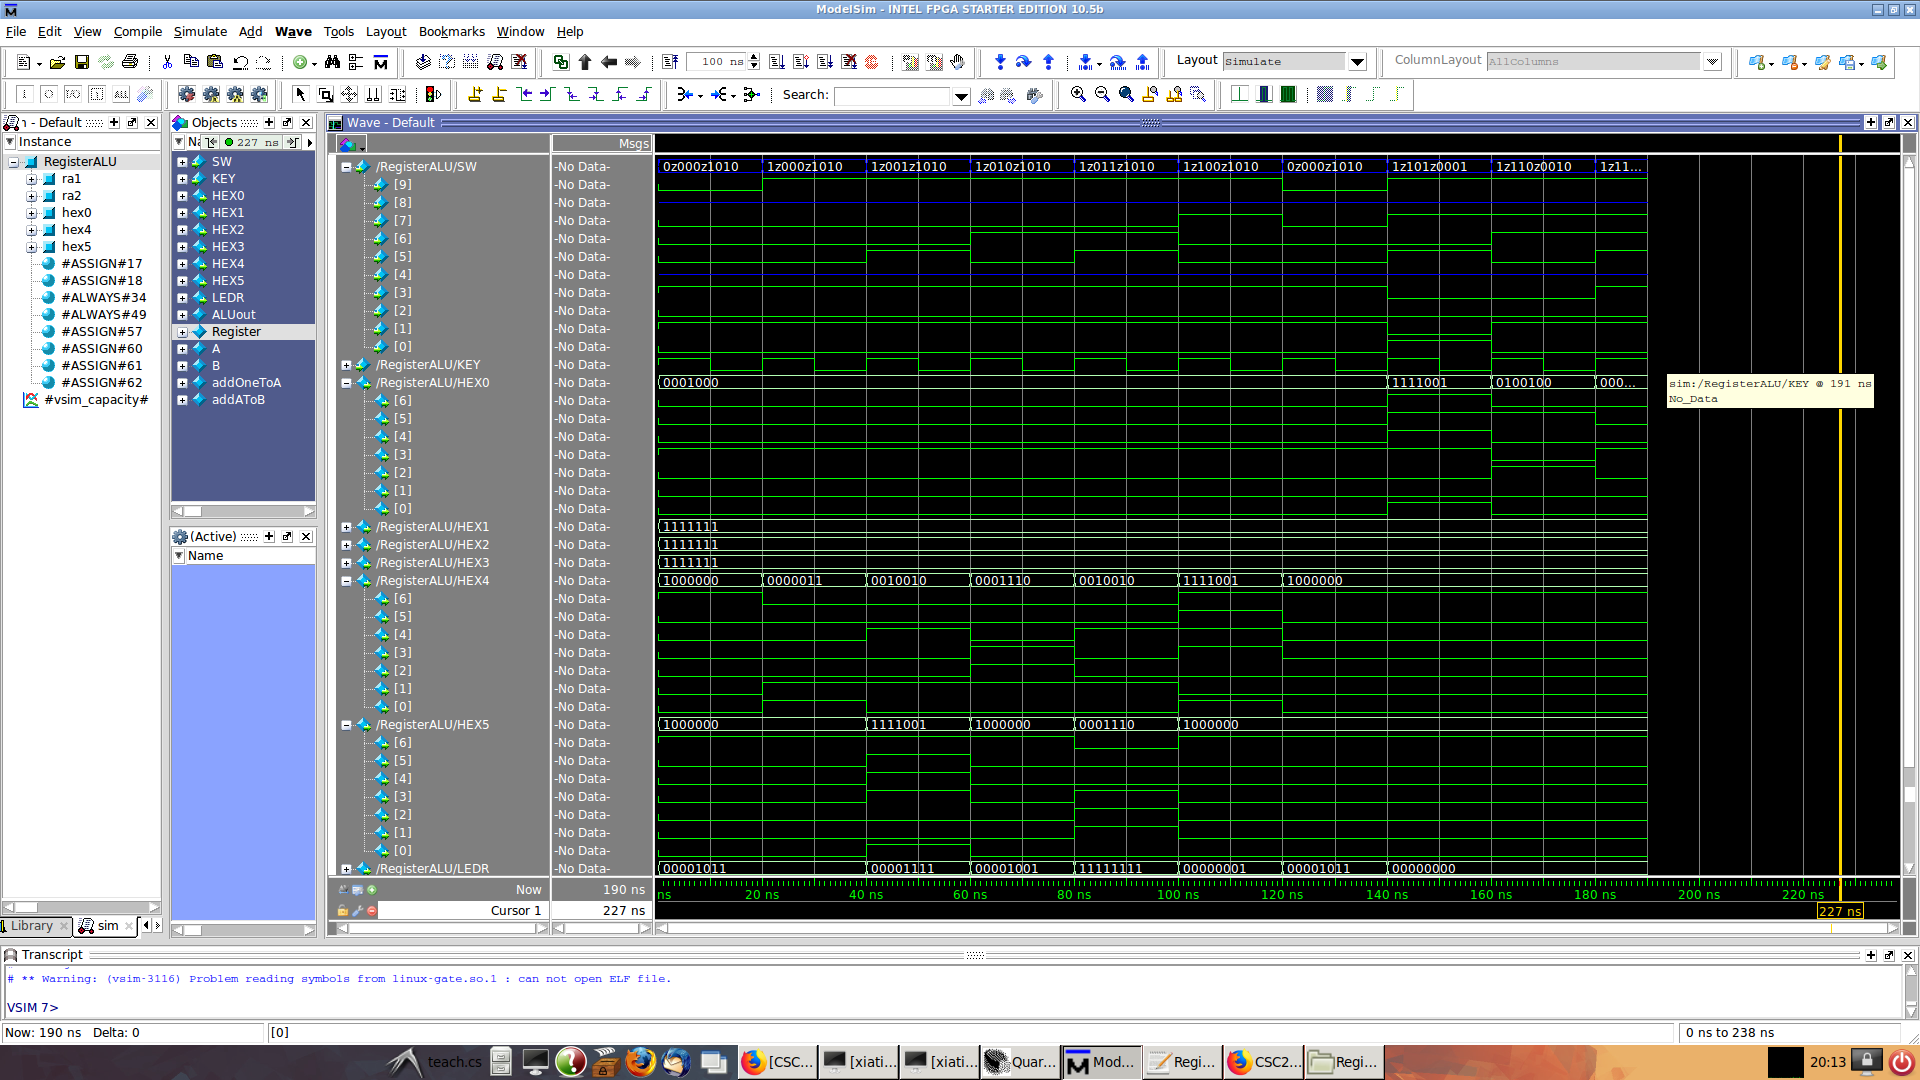
\includegraphics[scale=0.22]{pt2_hex_displays.png}
    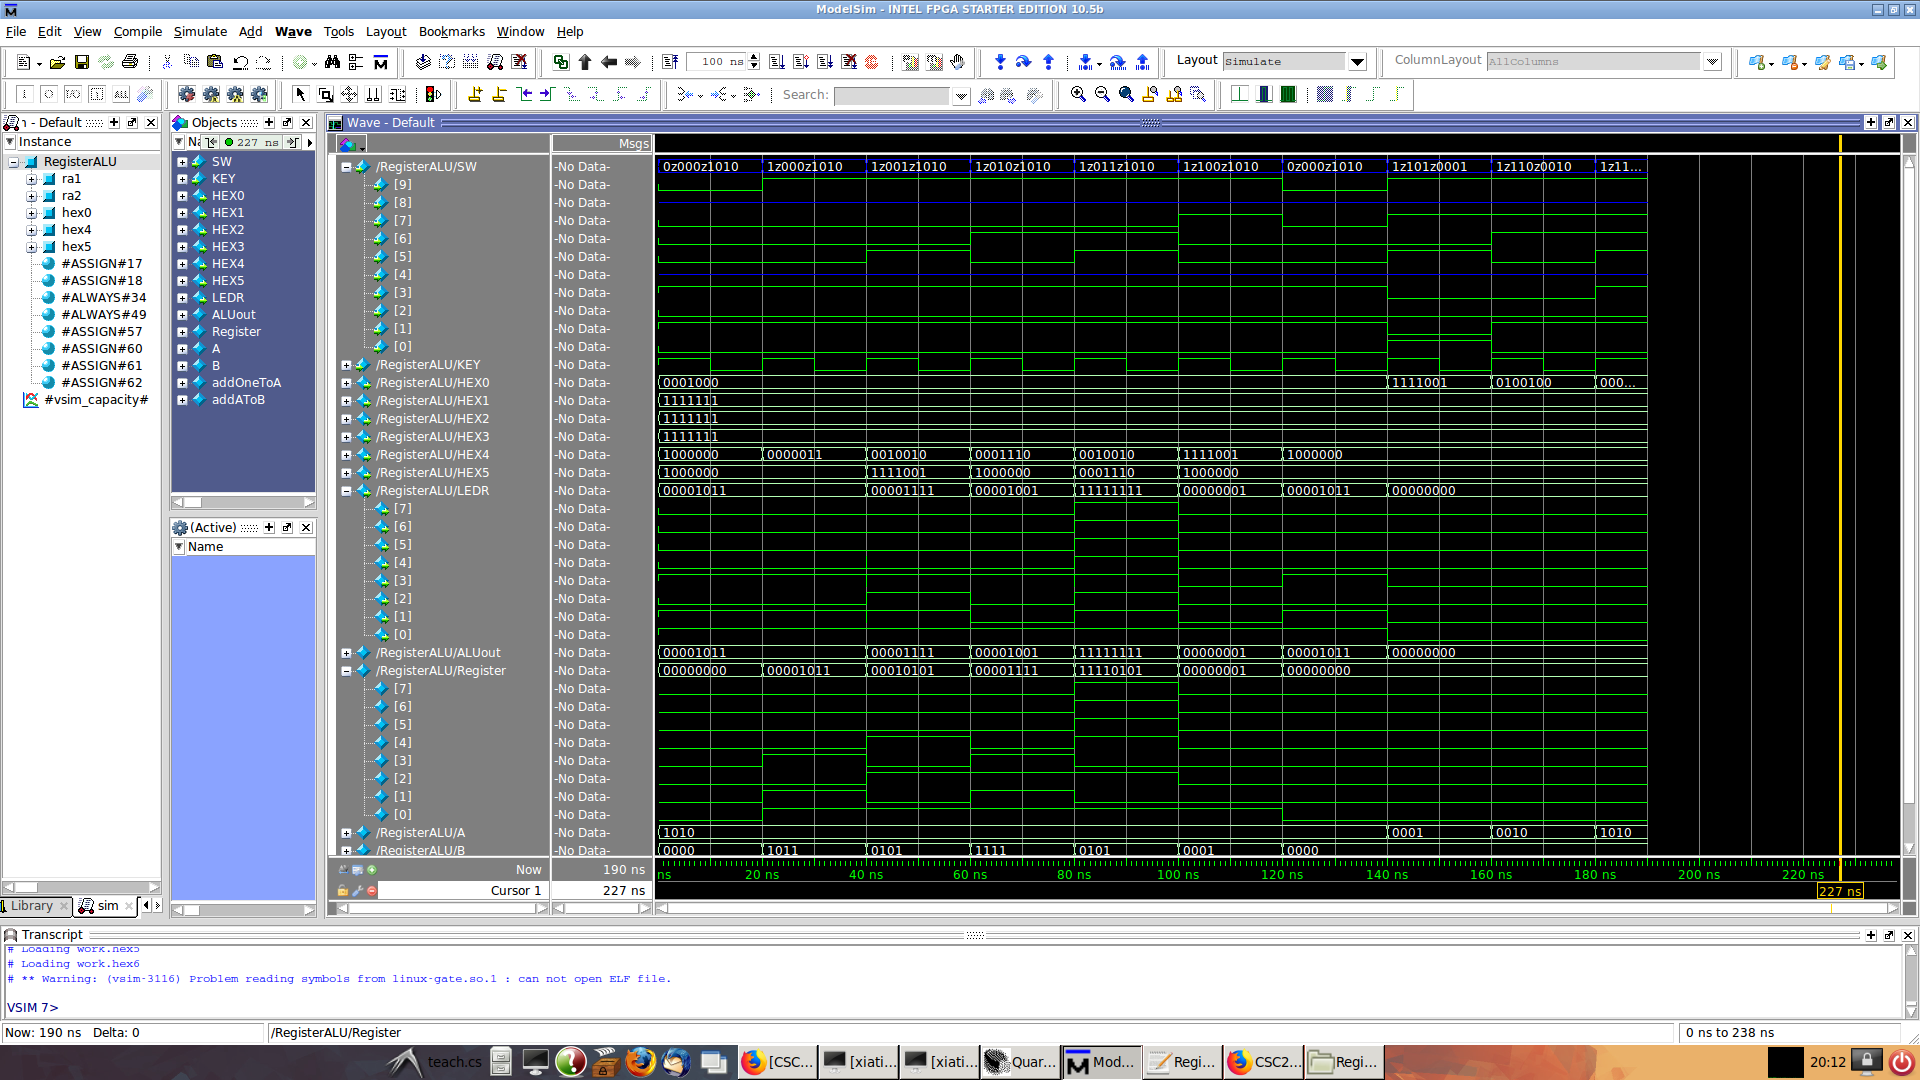
\includegraphics[scale=0.22]{pt2_led_register.png}
\end{center}

\section*{PART III}
\paragraph{1.} If \texttt{load\_n = 1} and \texttt{ShiftRight = 0}, then the 
register remains unchanged during the entire process. Since \texttt{ShiftRight}
is connected to the \texttt{shift} input of each ShifterBit and this essentially 
feed back the register with its own value. 
\paragraph{2.} Here is my schematic:
\begin{center}
    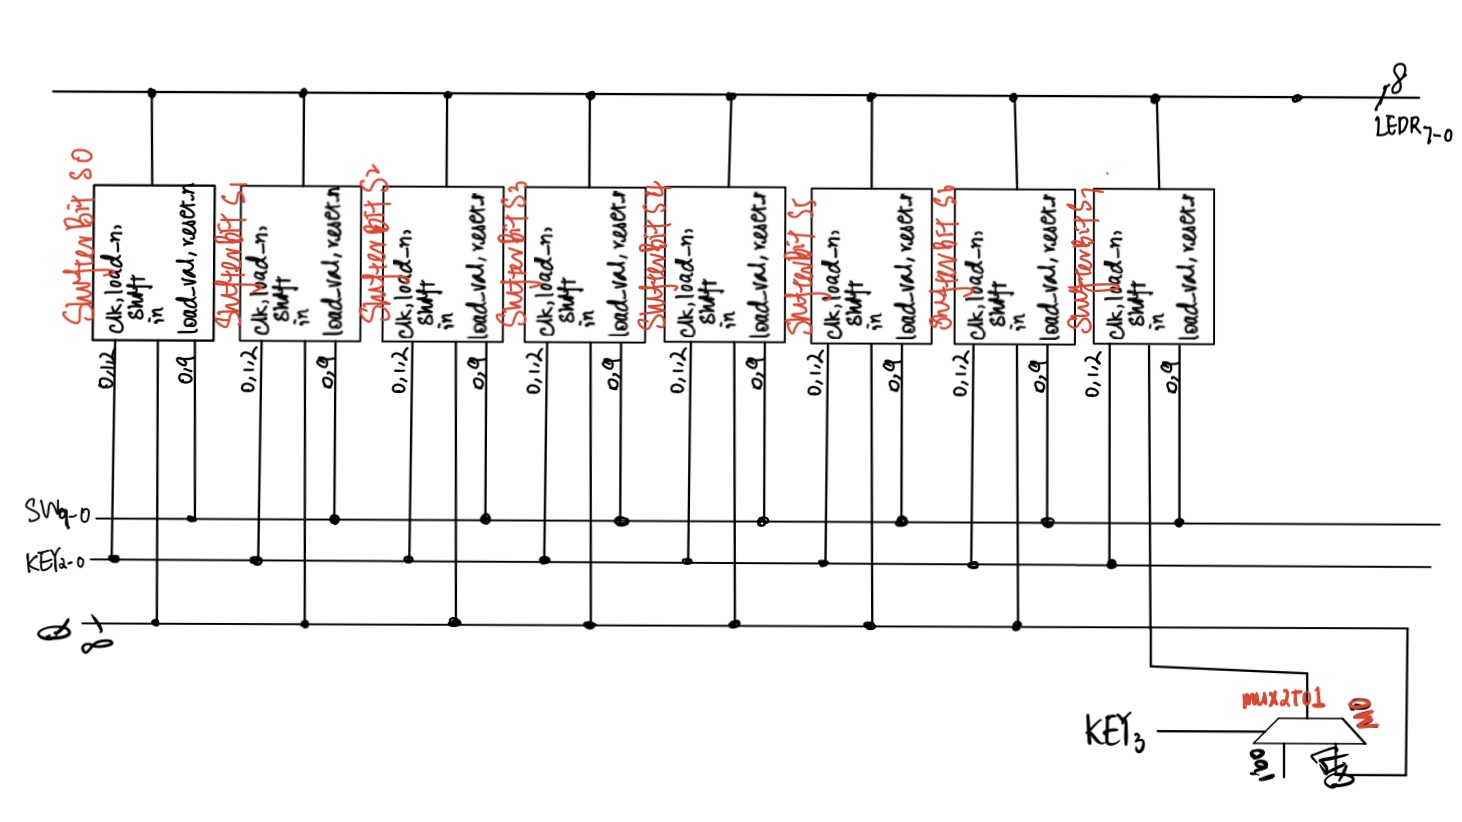
\includegraphics[scale=0.3]{q3_scheme.jpg}
\end{center}
\paragraph{4.} Here is my verlog code for Shifter:
\begin{minted}{verilog}
    module RegisterShifter(SW, KEY, LEDR);
        input [9:0] SW; // SW8 Unused
        input [3:0] KEY;
        output [7:0] LEDR;
        
        ShifterUnit8 s(
            // SW7-0: LoadVal
            .LoadVal(SW[7:0]),
            // KEY[1] Load_n
            .Load_n(KEY[1]),
            // KEY[2] ShifterRight
            .ShiftRight(KEY[2]),
            // KEY[3] ASR
            .ASR(KEY[3]),
            // KEY[0] Clock Signal
            .clk(KEY[0]),
            // Reset or not
            .reset_n(SW[9]),
            .q(LEDR[7:0])
        );
    endmodule


    // 8 bit shifter module
    module ShifterUnit8(LoadVal, Load_n, ShiftRight, ASR, clk, reset_n, q);
        input [7:0] LoadVal;
        input Load_n, ShiftRight, ASR, clk, reset_n;
        output [7:0] q;
        
        wire w0;
        
        ASRController asr0(
            .asr(ASR),
            .first(LoadVal[7]),
            .m(w0)
        );
        
        ShifterBit s7(
            .load_val(LoadVal[7]),
            .load_n(Load_n),
            .shift(ShiftRight),
            .clk(clk),
            .reset_n(reset_n),
            .in(w0),
            .out(q[7])
        );
        
        ShifterBit s6(
            .load_val(LoadVal[6]),
            .load_n(Load_n),
            .shift(ShiftRight),
            .clk(clk),
            .reset_n(reset_n),
            .in(q[7]),
            .out(q[6])
        );
        
        ShifterBit s5(
            .load_val(LoadVal[5]),
            .load_n(Load_n),
            .shift(ShiftRight),
            .clk(clk),
            .reset_n(reset_n),
            .in(q[6]),
            .out(q[5])
        );
        
        ShifterBit s4(
            .load_val(LoadVal[4]),
            .load_n(Load_n),
            .shift(ShiftRight),
            .clk(clk),
            .reset_n(reset_n),
            .in(q[5]),
            .out(q[4])
        );
        
        ShifterBit s3(
            .load_val(LoadVal[3]),
            .load_n(Load_n),
            .shift(ShiftRight),
            .clk(clk),
            .reset_n(reset_n),
            .in(q[4]),
            .out(q[3])
        );
        
        ShifterBit s2(
            .load_val(LoadVal[2]),
            .load_n(Load_n),
            .shift(ShiftRight),
            .clk(clk),
            .reset_n(reset_n),
            .in(q[3]),
            .out(q[2])
        );
        
        ShifterBit s1(
            .load_val(LoadVal[1]),
            .load_n(Load_n),
            .shift(ShiftRight),
            .clk(clk),
            .reset_n(reset_n),
            .in(q[2]),
            .out(q[1])
        );
        
        ShifterBit s0(
            .load_val(LoadVal[0]),
            .load_n(Load_n),
            .shift(ShiftRight),
            .clk(clk),
            .reset_n(reset_n),
            .in(q[1]),
            .out(q[0])
        );

    endmodule

    // Acts like a mux2to1: ASR or not
    module ASRController(asr, first, m);
        input asr, first;
        output m;
        reg out;
        always @(*)
        begin
            if (asr == 1'b1)
                out = first;
            else
                out = 1'b0;
        end
        assign m = out;
    endmodule

    module ShifterBit(load_val, load_n, clk, reset_n, shift, in, out);
        input load_val, load_n, clk, reset_n, shift, in;
        output out;
        wire w0;
        wire w1;
        
        mux2to1 m0(
            .x(out),
            .y(in),
            .s(shift),
            .m(w0)
        );
        
        mux2to1 m1(
            .x(load_val),
            .y(w0),
            .s(load_n),
            .m(w1)
        );
        
        DFlipFlop d0(
            .d(w1),
            .clk(clk),
            .r(reset_n),
            .q(out)
        );

    endmodule

    // mux2to1 from lab2
    module mux2to1(x, y, s, m);
        input x; //selected when s is 0
        input y; //selected when s is 1
        input s; //select signal
        output m; //output
        
        assign m = s & y | ~s & x;
    endmodule

    module DFlipFlop(d, clk, r, q);
        input d, clk;
        input r;
        output q;
        
        reg q;
        
        always @(posedge clk)
        begin
            // If reset_n == 0: reset the flip flop
            if (r == 1'b0)
                q <= 1'b0;
            // transparent d-flipflop
            else
                q <= d;
        end
    endmodule
\end{minted}

\paragraph{5.} Here are screen shots for the model sim results
\begin{center}
    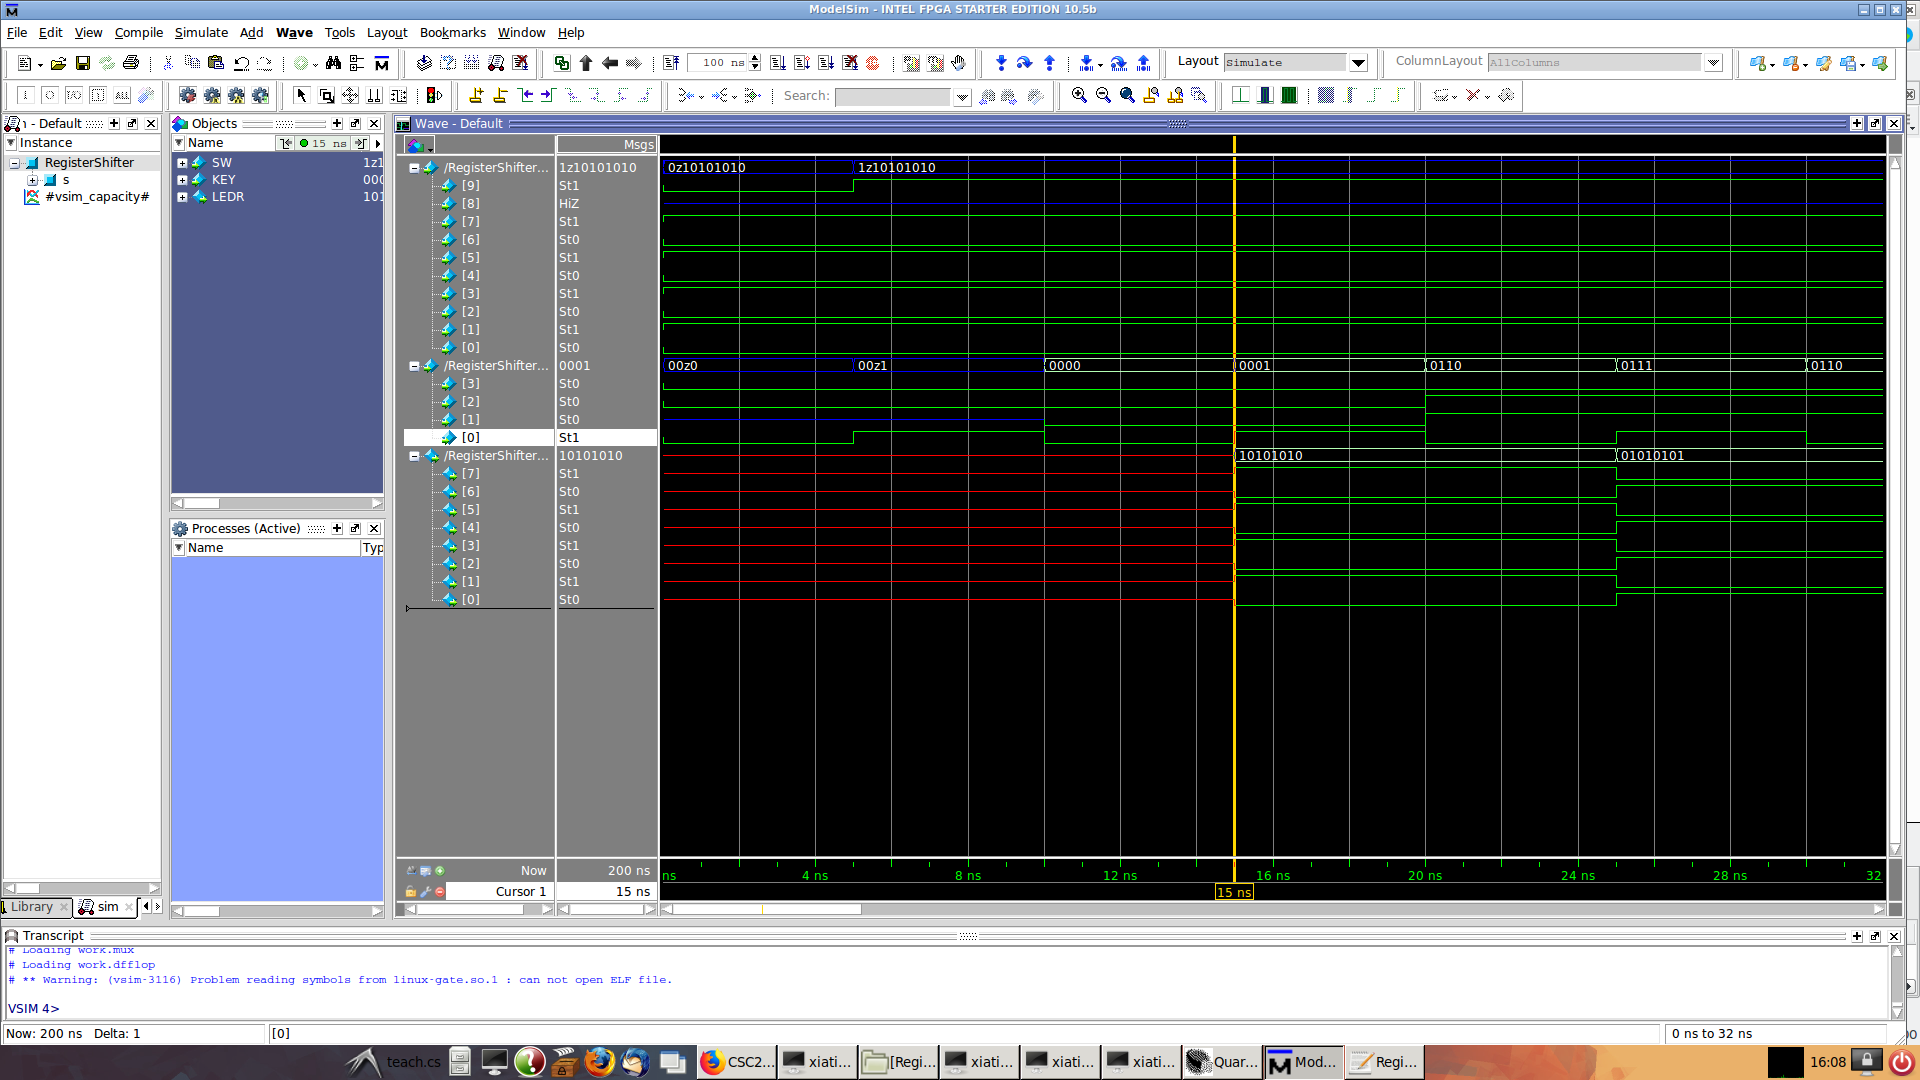
\includegraphics[scale=0.22]{not_reset.png}
    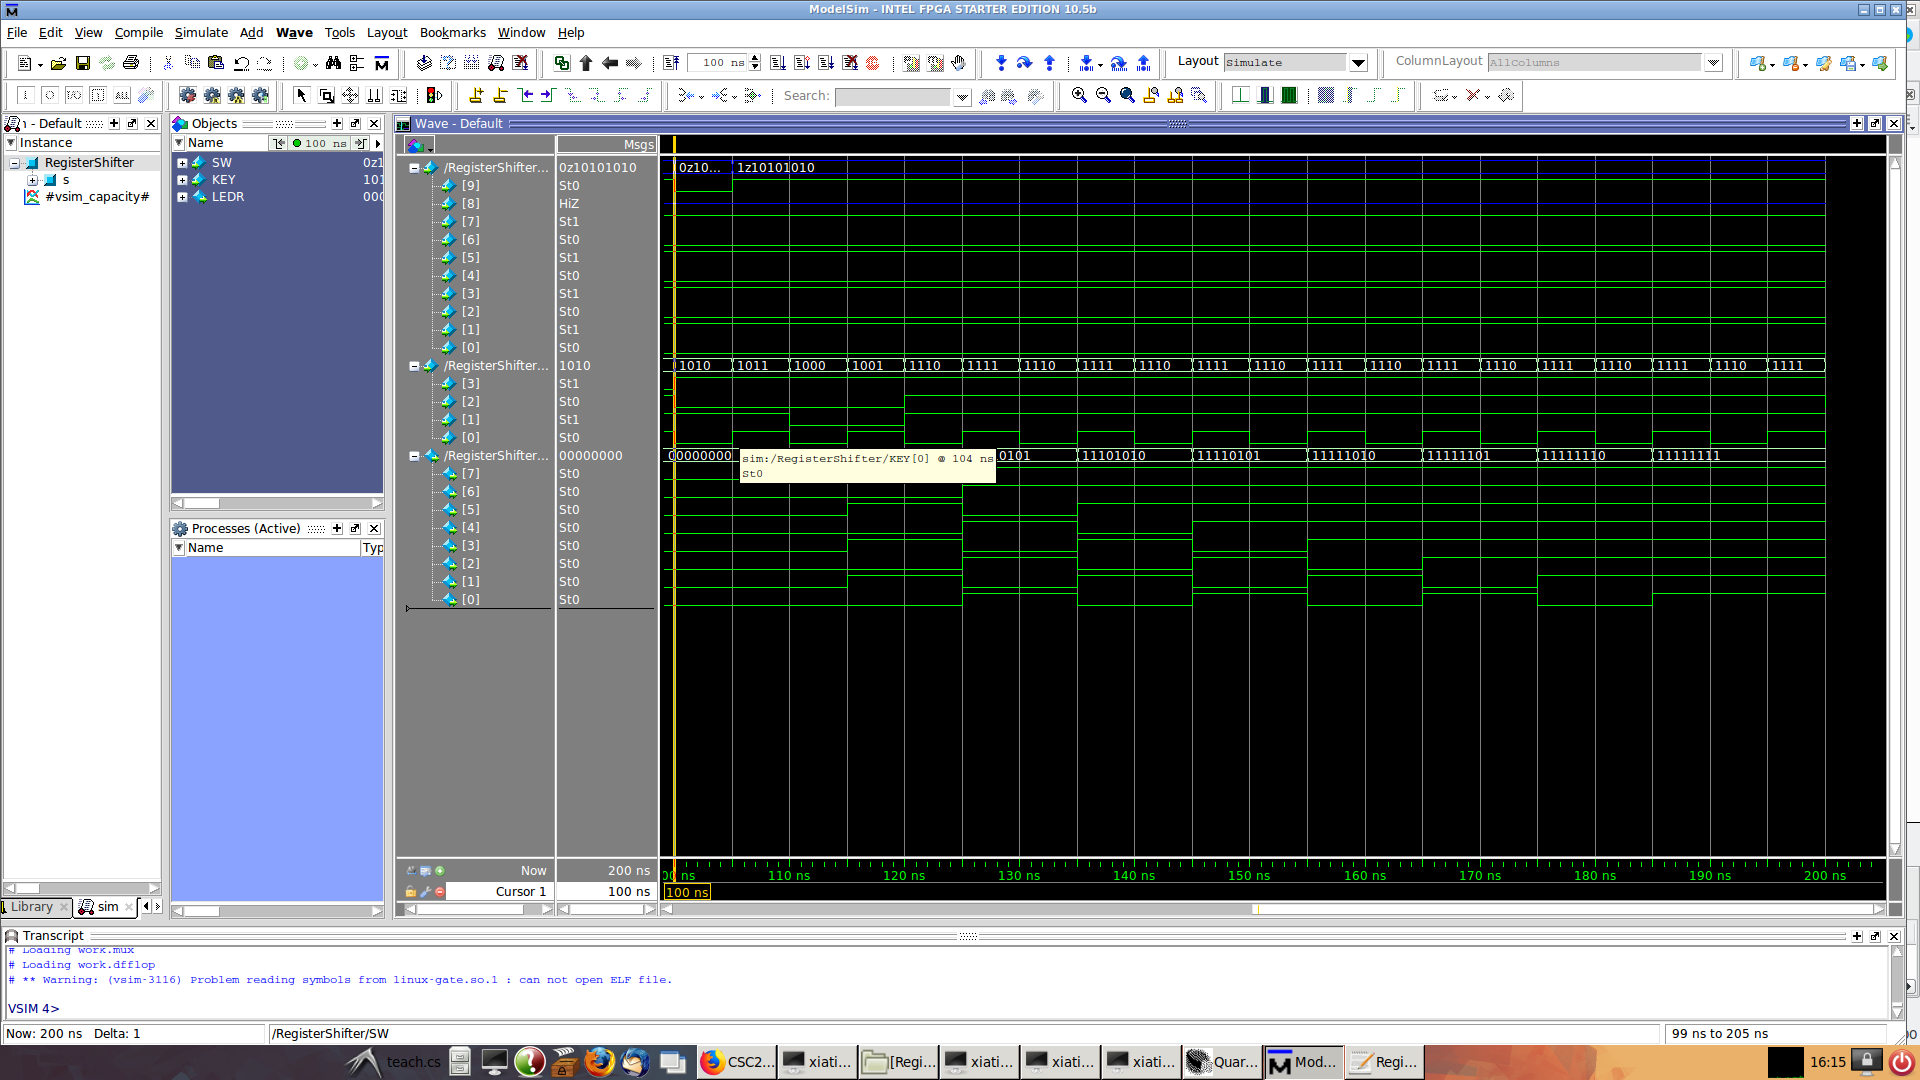
\includegraphics[scale=0.22]{asr.png}
    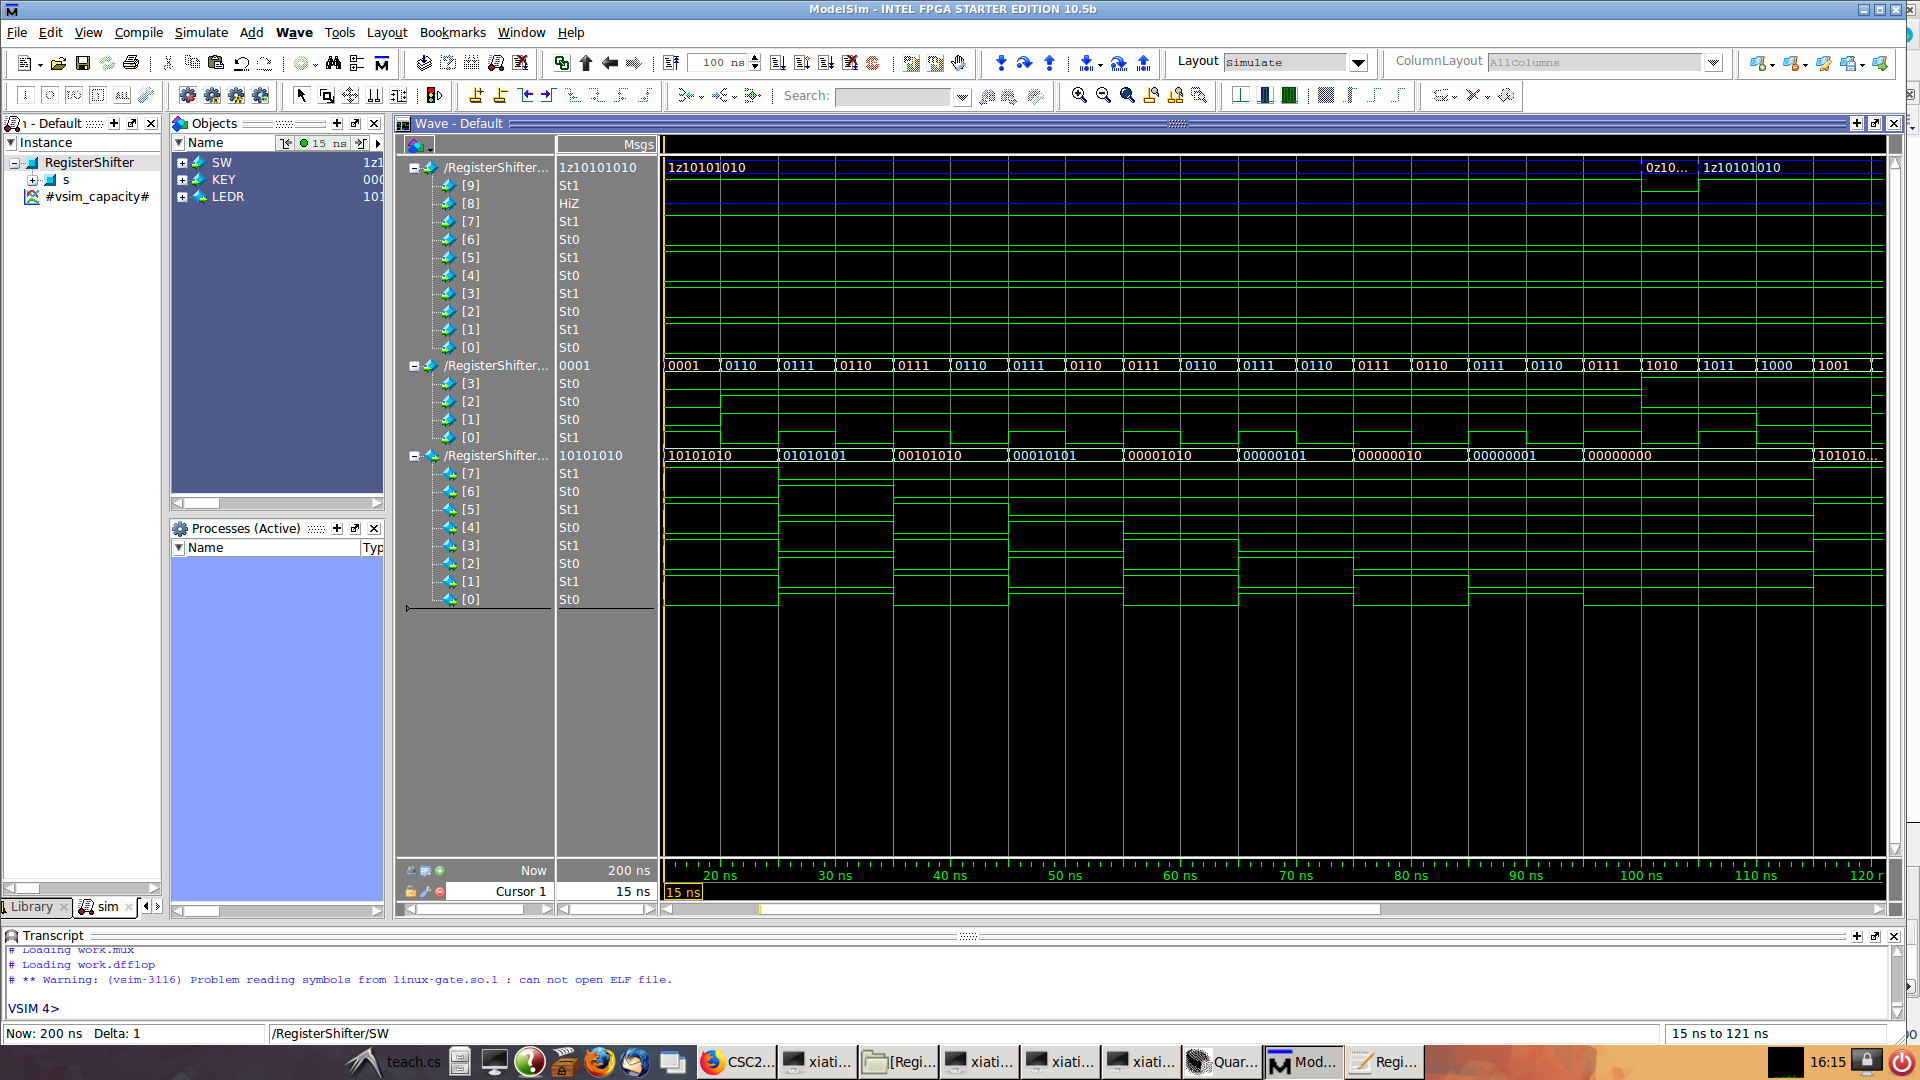
\includegraphics[scale=0.22]{non_asr.png} 
\end{center}
\end{document}
